\documentclass[12pt]{article}
% Font and language
\usepackage{fontspec}
\usepackage{polyglossia}
\setmainlanguage{greek}
\setotherlanguage{english}
\setmainfont{Linux Libertine O}
\newfontfamily\greekfont[Script=Greek]{Linux Libertine O}
\newfontfamily\greekfontsf[Script=Greek]{Linux Libertine O}
\newfontfamily\greekfonttt[Script=Greek]{Linux Libertine O}

% Paper
\usepackage[a4paper]{geometry}

% Images
\usepackage{graphicx}
\graphicspath{\subfix{./images/}}

% Links
\usepackage{hyperref}
\hypersetup{
	colorlinks=true,
	linkcolor=black,
	citecolor=black,
	urlcolor=blue,
}

% Figure numbering
\usepackage{chngcntr}
\counterwithin{figure}{section}

% Multifiles project
\usepackage{subfiles}

% Tables
\usepackage{array}
\usepackage{tabulary}
\usepackage{float}
\usepackage{multirow}
\usepackage{xstring}
\usepackage{longtable}

% Math
\usepackage{bm}
\usepackage{amsmath}
\newcommand{\tsub}[1]{\texttt{\tiny#1}}

\title{
	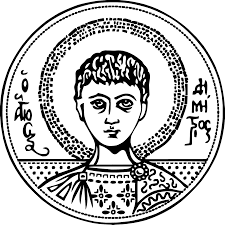
\includegraphics[height=3cm]{auth.png}\\
	\large{Αριστοτέλειο Πανεπιστήμιο Θεσσαλονίκης}\\
	\large{Τμήμα Ηλεκτρολόγων Μηχανικών και Μηχανικών Υπολογιστών}\\
	\vspace{2cm}
	\LARGE{Βάσεις Δεδομένων}\\
	\LARGE{GoT-DB}\\
	\vspace{0.5cm}
	\large{9\textsuperscript{o} Εξάμηνο}\\
	\vspace{3cm}
}

\author{
	\underline{Ομάδα 24}\\
	Γιώργος Κούκας		9486\\
	\href{mailto:istefanidi@auth.gr}{Στεφανίδης Ιωάννης} 9587\\
	Σφυράκης Εμμανουήλ 9507
	\vspace{3cm}
}

   
\begin{document}
\pagenumbering{gobble} % to remove numbering for first page
\maketitle \newpage
\pagenumbering{arabic}
\tableofcontents \newpage
\listoffigures
\listoftables
\newpage

\section{Εισαγωγή}
\subfile{sections/intro}

\section{Κατηγορίες Χρηστών και Απαιτήσεις τους}
\subfile{sections/user_categories}

\section{Μοντέλο Οντοτήτων/Συσχετίσεων}
\subfile{sections/entity_model}

\section{Σχεσιακό Μοντέλο}
\subfile{sections/relational_model}

\section{Παραδείγματα}
\subfile{sections/examples}


\section{Σημειώσεις}
Τον κώδικα όλου του πρότζεκτ μπορείτε να τον βρείτε στο \href{https://github.com/johnstef99/GoT-db-auth}{github}.
Το mysql-workbench model έγινε μετά από reverse engineer του schema που φτιάξαμε
μέσω του Laravel framework. Για αυτόν τον λόγο θα βρείτε σε κάθε table τα
columns \verb|created_at, updated_at| που είναι τα λεγόμενα timestamps του
Laravel.

Τα views στην βάση δημιουργήθηκαν "με το χέρι", δηλαδή δεν βρίσκονται μέσα στο
Laravel project. Το SQL script για την δημιουργία τους υπάρχει μέσα στο dump της
gotdb.

\begin{figure}[H]
	\centering
	\begin{tabular}{l l}
		\textbf{Database}: & \verb|mariadb 15.1 Distrib 10.6.5-MariaDB| \\
		\textbf{PHP}:      & \verb|PHP 7.4.26|
	\end{tabular}
	\caption{Λογισμικό που χρησιμοποιήθηκε}
\end{figure}

\end{document}
